% \documentclass[draft]{beamer}
\documentclass{beamer}
% \documentclass[24pt, a0papper, landscape]{tikzposter}

%
%
% velikost papiru
% nazev posteru a autori
% sirka hlavnich sloupcu
%
%



\usepackage{beamerposter}

% \setlength{\paperwidth}{130.0cm}
% \setlength{\paperheight}{80.0cm}
% \setlength{\textwidth}{128.0cm}
% \setlength{\textheight}{78.0cm} 


% \setlength{\paperwidth}{1500mm}
% \setlength{\paperheight}{800mm}
% \setlength{\textwidth}{1470mm}
% \setlength{\textheight}{770mm} 


% A0
% 841 x 1189 mm
\setlength{\paperwidth}{1250mm}
\setlength{\paperheight}{841mm}
\setlength{\textwidth}{1240mm}
\setlength{\textheight}{830mm} 




% \usepackage{fontspec}
% +\newfontfamily\myfont[phv]{Helvetica}



% \usepackage[scale=1.24]{beamerposter} 
% \usepackage{caption}
% \captionsetup{font=scriptsize,labelfont=scriptsize}
\usepackage[utf8]{inputenc}

% \usepackage[czech]{babel}
\usepackage[english]{babel}   



% \usepackage[font={small,it,rf}]{caption}
\setbeamertemplate{caption}[numbered]{}
% \usepackage{caption}
% \captionsetup{font=scriptsize,labelfont=scriptsize}

% \usepackage{caption}
% 
% 
% \usepackage{subcaption}

\usepackage{wrapfig}
\usepackage{listings}


\usepackage{multicol}
% \usepackage[cp1250]{inputenc}
% \usepackage[czech]{babel}
\usepackage{natbib}
% \bibliographystyle{agsm}
\bibliographystyle{apalike}
\usepackage{tabularx}



\usepackage{ragged2e}



\renewcommand{\thesubsection}{\thesection.\arabic{subsection}}


\usetheme{confposter}

\setbeamercolor{block title}{fg=nblue,bg=white} % Colors of the block titles
\setbeamercolor{block body}{fg=black,bg=white} % Colors of the body of blocks
\setbeamercolor{block alerted title}{fg=white,bg=dblue!70} % Colors of the highlighted block titles
\setbeamercolor{block alerted body}{fg=black,bg=dblue!10} % Colors of the body of highlighted blocks
% Many more colors are available for use in beamerthemeconfposter.sty

%-----------------------------------------------------------
% Define the column widths and overall poster size
% To set effective sepwid, onecolwid and twocolwid values, first choose how many columns you want and how much separation you want between columns
% In this template, the separation width chosen is 0.024 of the paper width and a 4-column layout
% onecolwid should therefore be (1-(# of columns+1)*sepwid)/# of columns e.g. (1-(4+1)*0.024)/4 = 0.22
% Set twocolwid to be (2*onecolwid)+sepwid = 0.464
% Set threecolwid to be (3*onecolwid)+2*sepwid = 0.708


\newcommand{\separacnisloupec}{
\begin{column}{0.02\linewidth}
\centering
\begin{beamercolorbox}[wd=0.25cm,dp=0.95\textheight]{cboxb}\end{beamercolorbox}
\end{column}
} % Empty spacer column


\newcommand{\separacnisloupecc}{
\begin{column}{0.02\linewidth}
\centering
\begin{beamercolorbox}[wd=0.125cm,dp=0.45\textheight]{cboxb}\end{beamercolorbox}
\end{column}
} % Empty spacer column



\newlength{\sepwid}
% 
\newlength{\lcolwid}
\newlength{\rcolwid}
\newlength{\mezerapopisek}

\newlength{\oneprvni}
\newlength{\twodruhy}
\newlength{\threetreti}


\setlength{\sepwid}{0.02\paperwidth} % Separation width (white space) between columns
\setlength{\oneprvni}{0.26\paperwidth} % Width of one column
\setlength{\twodruhy}{0.38\paperwidth} % Width of two columns
\setlength{\threetreti}{0.28\paperwidth} % Width of three columns




\setlength{\lcolwid}{0.5438\paperwidth} % Width of left column
\setlength{\rcolwid}{0.3361\paperwidth} % Width of right column

\setlength{\mezerapopisek}{-9pt} % Width of right column
%-----------------------------------------------------------


\usepackage{graphicx}  % Required for including images

\usepackage{booktabs} % Top and bottom rules for tables

%----------------------------------------------------------------------------------------
%       TITLE SECTION \usepackage[font=scriptsize]{caption}
%----------------------------------------------------------------------------------------

\title
{
Could be hydrological model parameters inferred from a soil texture?
}



\author{{\bf \Large Martin Landa} (\href{mailto:martin.landa@fsv.cvut.cz}{martin.landa@fsv.cvut.cz}), 
Peter Kavka,
Jakub Je\v{r}{\'a}bek,
Barbora J{\'a}chymov{\'a}} % Author(s)

\institute{Department of Irrigation, Drainage and Landscape Engineering, Faculty of Civil Engineering, Czech Technical University in Prague, Czech Republic } % Institution(s)

%----------------------------------------------------------------------------------------




\newcommand{\mojesekce}[1]{
\section{asdfasdfa}
\begin{center}
\begin{beamercolorbox}[rounded = true, ht = 3ex, dp={0.5ex}]{myblocktitle2}
 {\bf\large\rmfamily\thesection\hspace{1cm}#1}
\end{beamercolorbox}
\end{center}
\vspace{-1.2cm}
}

\newcommand{\mojesekcee}[1]{
\section{asdfasdfa}
\begin{center}
\begin{beamercolorbox}[rounded = true, ht = 6ex, dp={0.5ex}]{myblocktitle2}
 {\bf\large\rmfamily\thesection\hspace{1cm}#1}
\end{beamercolorbox}
\end{center}
}

%  kvuli flow chart
\usepackage{tikz}
\usetikzlibrary{shapes.geometric, arrows}
\tikzstyle{startstop} = [rectangle, rounded corners, minimum width=3cm, minimum height=1cm,text centered, draw=black, fill=red!30]
\tikzstyle{io} = [trapezium, trapezium left angle=70, trapezium right angle=110, minimum width=1cm, minimum height=1cm, text centered, draw=black, fill=blue!30]
\tikzstyle{arrow} = [thick,->,>=stealth]
\tikzstyle{decision} =  [diamond, minimum width=1cm, minimum height=1cm, text centered, text width=2cm, draw=black, fill=green!30, aspect=2]
\tikzstyle{process} = [rectangle, minimum width=3cm, minimum height=1cm, text centered, text width=3cm, draw=black, fill=orange!30]
\tikzstyle{guide} = [inner sep=0pt,minimum size=0mm]
\tikzstyle{line} = [thick]





\usepackage{color}

\newcommand*{\mathcolor}{}
\def\mathcolor#1#{\mathcoloraux{#1}}
\newcommand*{\mathcoloraux}[3]{%
  \protect\leavevmode
  \begingroup
    \color#1{#2}#3%
  \endgroup
}


\begin{document}

%  \addtobeamertemplate{block end}{}{\vspace*{2ex}} % White space under blocks
% \addtobeamertemplate{block alerted end}{}{\vspace*{2ex}} % White space under highlighted (alert) blocks
% 
% \setlength{\belowcaptionskip}{2ex} % White space under figures
% \setlength\belowdisplayshortskip{2ex} % White space under equations

\begin{frame}[t]

\begin{columns}[t] 
  
  \begin{column}{\sepwid}\end{column}
  
  
  \begin{column}{\oneprvni} 
    % \begin{columns}
%     \begin{column}{0.5\textwidth}
%     
%     \end{column}
% \end{columns}
% \begin{columns}
%     \begin{column}{0.5\textwidth}
%     
%     \end{column}
% \end{columns}

%   \begin{wrapfigure}[8]{r}{0.4\textwidth}
%     \begin{minipage}{\dimexpr\linewidth-2\fboxrule-2\fboxsep}
%     {\tiny
%     \begin{lstlisting}
%        @ @ @   @       @     @ @     @ @ @     @ @ @ @  @ @ @    @ @ @
%       @        @ @   @ @   @     @   @     @   @        @     @  @     @
%       @        @   @   @  @       @  @      @  @        @     @  @     @
%         @ @    @       @  @       @  @      @  @ @ @    @ @ @    @ @ @
%             @  @       @  @       @  @      @  @        @   @    @
%             @  @       @   @     @   @     @   @        @    @   @
%        @ @ @   @       @     @ @     @ @ @     @ @ @ @  @     @  @
% 
%       \  \  /   / /    \   \  /   \  /    /     /        @ @ @   @ @ @
%        \ _\/   /_/      \   \/     \/    /_____/        @     @  @     @
%            \__/          \  /      _\___/                     @  @      @
%                \____      \/      /                          @   @      @
%                     \_____/______/                         @     @      @
%                                  \                       @       @     @
%                                   \____________________ @ @ @ @  @ @ @
%     \end{lstlisting}
%     }
%     \end{minipage}
%   \end{wrapfigure}
%----------------------------------------------------------------------------------------
%   Summary
%----------------------------------------------------------------------------------------



\begin{alertblock}{Summary}
    {\large
    \begin{itemize}
        \item Parameters of surface runoff model were derived for each soil texture (past work)
        \item Newly the parameters were derived with optimization on extended set of data
        \item Sensitivity analysis were performed 
        \item Uncertainly of parameters were assessed with Monte Carlo simulations 
        \item New open source model provider is presented 
    %       \item
    %       \item
    \end{itemize}
    }
%     In the past parameters of the phy\-sically-based, distributed, event runoff/erosion SMODERP2D Model were inferred for each soil textural class. This approach were performed to simplify practitioners life since the parameters were ready to use if one have the soil texture of the area of interest. In order to assess variability of each parameter within and across textural classes the model were optimized to laboratory artificial rainfall experiments at 4 different textural classes. 
%     Results shows that ...
\end{alertblock}\vspace{0.9cm}



%----------------------------------------------------------------------------------------
%   INTRODUCTION
%----------------------------------------------------------------------------------------


\mojesekce{Material and Methods}
\subsection{Model structure}
\begin{block}{Model structure}
    Based on a balance equation 
    $$
        \frac{Storage}{\Delta t} = \nonumber  
        Inflow - Outflow
    $$
    is inferred bucket model with kinematic wave approach for momentum 
    $$
%       \begin{split}
        \frac{\partial h_{i}}{\partial t} =  es_{i} + \sum_j^n q_{j} - inf_{i} - q_{i} - ret_i
    $$
    where $h$ is water level [$L$], $es$ is effective precipitation [$L.T^{-1}$], $inf$ is infiltration [$L.T^{-1}$], $ret$ surface retention [$L$], and $q$ is the Manning-Strickler formula
    \begin{equation}
      q = Xi^Yh^b. 
      \label{eq:manning}
    \end{equation}

    {\bf Parameters $X$, $Y$, and $b$ were inferred for each soil textural class.} Variability of those parameters within and among textural classes is assessed in this poster. Infiltration is solved with Phillip's infiltration equation:
    \begin{equation}
      inf = 1/2St^{-1/2} + Ks.
      \label{eq:Phillips}
    \end{equation}
    {\bf Saturated hydraulic conductivity $Ks$ [$L.T^{-1}$] and sorptivity $S$ [$L.T^{-1/2}$] were fitted with measured data.}
\end{block}



\subsection{Actual parameter values}
\begin{block}{Actual parameter values}\vspace{-1cm}
\begin{columns}
    \begin{column}{0.25\textwidth}
        Actual parameter values were inferred based on @@@(petr s referenci)
    \end{column}
    \begin{column}{0.75\textwidth}
        \begin{table}[]
            \small
            \caption{Current parameter set for soil textural classes}
            \begin{tabular}{lllll|lllll}
            \hline
            \hline
            Textural class & ID  & $b$    & $X$    & $Y$     & Textural class  & ID   & $b$    & $X$    & $Y$  \\
            \hline
            sand           & SS  & 1.82 & 8.81 & 0.366 & sandy clay loam & SCL  & 1.7  & 10.7 & 0.603 \\
            loamy sand     & LS  & 1.82 & 8.81 & 0.366 & clay loam       & CL   & 1.7  & 10.7 & 0.603 \\
            sandy loam     & SL  & 1.79 & 9.2  & 0.462 & silty clay loam & SICL & 1.7  & 10.7 & 0.603 \\
            loam           & LL  & 1.74 & 10.1 & 0.561 & sandy clay      & SC   & 1.67 & 11.3 & 0.636 \\
            silt loam      & SIL & 1.74 & 10.1 & 0.561 & silty clay      & SIC  & 1.67 & 11.3 & 0.636 \\
            silt           & SI  & 1.74 & 10.1 & 0.561 & clay            & CC   & 1.67 & 11.3 & 0.636 \\
            \hline
            \hline
            \end{tabular}
        \end{table}
    \end{column}
\end{columns}
    
\end{block}

\subsection{Soil classes and ARE overview}
\begin{block}{Soil classes and ARE overview}
    \begin{itemize}
        \item 266 experiments with artificial rainfall were performed 
        \item Various slopes and rainfall intensities were tested for each location.
    \end{itemize}\vspace{-1cm}
% 
    \begin{columns}
        \begin{column}{0.4\textwidth}
            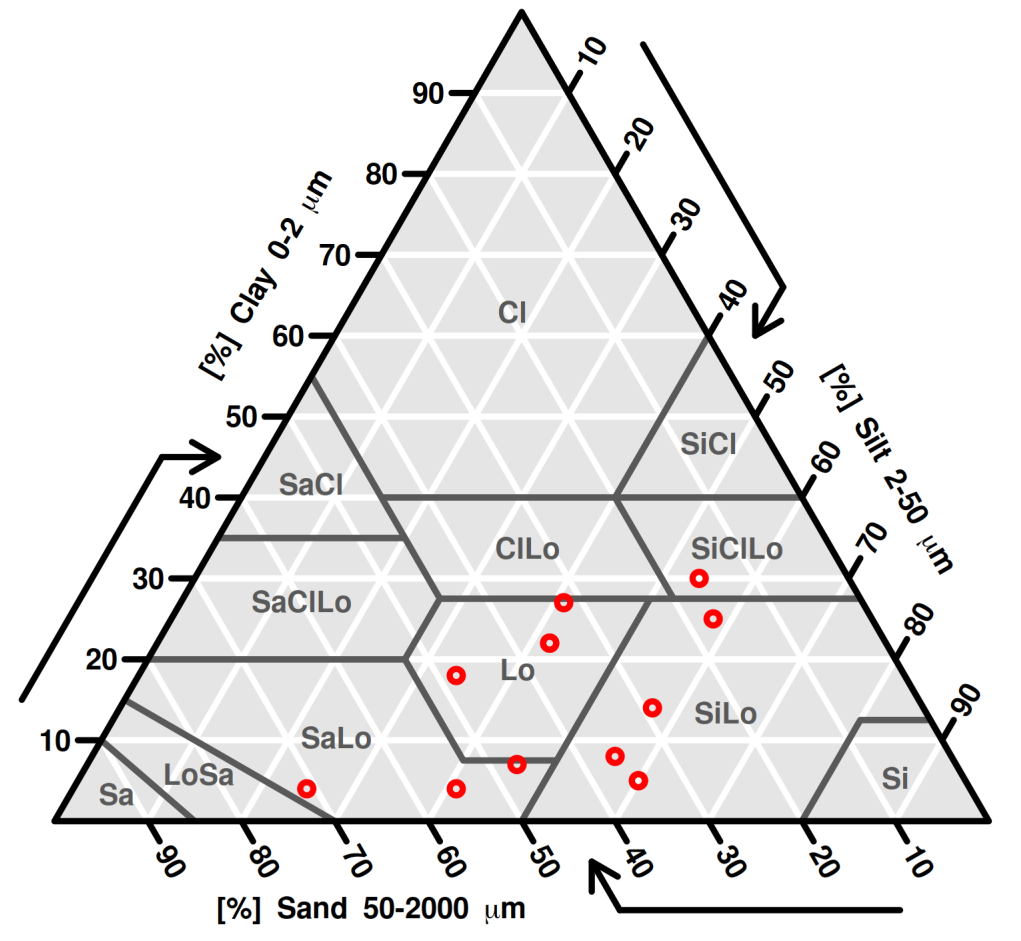
\includegraphics[width=.95\textwidth]{obr/soil_triangle.png}
        \end{column}
        \begin{column}{0.6\textwidth}
            {\small 
            \begin{table}[]
            \caption{Overview of artificial rainfall experimets}
                \begin{tabular}{lcccccc}
                \hline
                \hline
                location      & year    & no. of            & \multicolumn{3}{c}{soil texture {[}\%{]}}  & soil class      \\
                            &         & exper.       & clay  & silt  & sand &  \\
                \hline
                Horoměřice    & 2002    & 25                & 25             & 58            & 17            & silty loam      \\
                Třebsín I     & 2004    & 22                & 5              & 60            & 35            & silty loam      \\
                Neustupov     & 2006    & 14                & 4              & 41            & 55            & sandy loam      \\
                Klapý         & 2007    & 25                & 30             & 54            & 16            & silty clay loam \\
                Třebsín II    & 2008    & 28                & 5              & 60            & 35            & silty loam      \\
                Třebešice I   & 2009    & 27                & 4              & 25            & 71            & sandy loam      \\
                Třebešice II  & 2010    & 36                & 7              & 46            & 47            & sandy loam      \\
                Nučice        & 2011    & 35                & 14             & 57            & 29            & silty loam      \\
                Všetaty I     & 2012    & 24                & 22             & 42            & 36            & loam            \\
                Všetaty II    & 2013    & 17                & 22             & 42            & 36            & loam            \\
                Třebešice III & 2014    & 22                & 8              & 56            & 36            & silty loam      \\
                Nové Strašecí & 2015    & 20                & 27             & 41            & 32            & loam            \\
                Řisuty        & 2017    & 21                & 18             & 34            & 48            & loam           \\
                \hline
                \hline
                \end{tabular}
            \end{table}
            }
        \end{column}
    \end{columns}
\end{block}



        

  \end{column}


  \separacnisloupec


  \begin{column}{\twodruhy} 
    \mojesekce{Results}

\subsection{Sensitivity analyses}
\begin{block}{Sensitivity analyses}
\justifying
Each optimized parameter were increased and decreased with specific factor unit sum of squares increased with order of magnitude. 
\begin{columns}
    \begin{column}{0.4\textwidth}
        \begin{table}[]
            \begin{tabular}{lll}
                \hline
                \hline
                Paraneter & increase   & decrease \\
                          & factor (+) & factor (-) \\
                \hline
                X         & 80                  & 1/3.5               \\
                Y         & 1.3                 & 1/1.6               \\
                b         & 1.125               & 1/1.5               \\
                Ks        & 2.0                 & 1/5.0               \\
                S         & 2.0                 & 1/5.0               \\
                ret       & 1.5                 & 1/5.0              \\
                \hline
                \hline
            \end{tabular}
        \end{table}
    \end{column}
    \begin{column}{0.6\textwidth}
        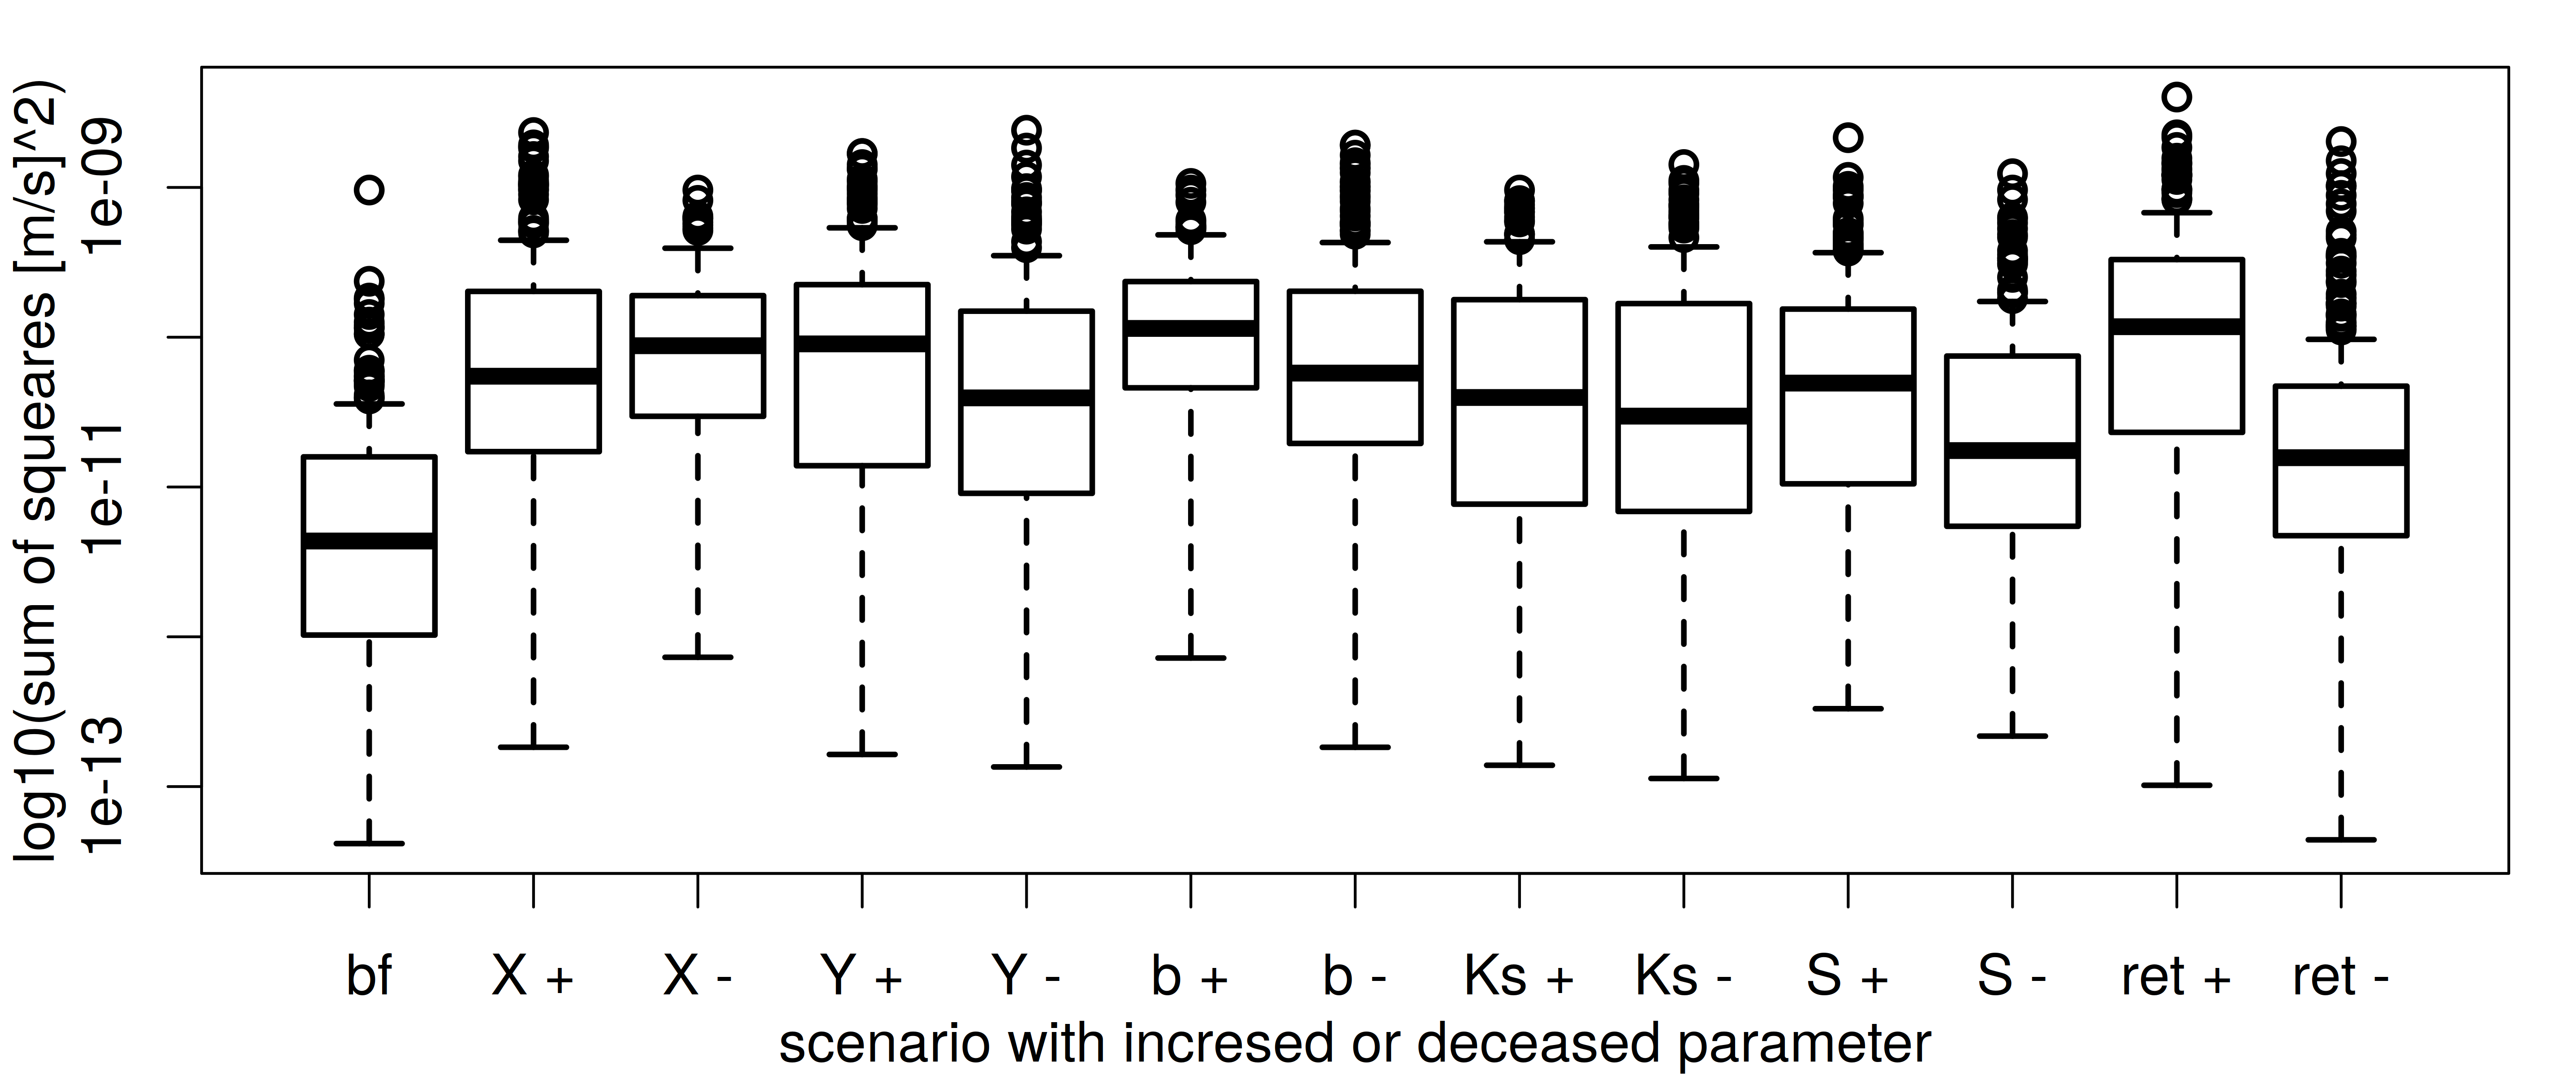
\includegraphics[width = \textwidth]{obr/sens.png}
    \end{column}
\end{columns}
\end{block}


\subsection{Model parameters and textural classes}
\begin{block}{Model parameters and textural classes}
\begin{columns}
    \begin{column}{0.2\textwidth}
    \end{column}
    \begin{column}{0.6\textwidth}

        \begin{table}[]
            \begin{tabular}{lllll}
            parameter: & X & Z & b & ret \\
            max & 30 & 5 & 4 & 0 \\
            min & 1 & 0.01 & 1 & -0.5 \\
            \end{tabular}
        \end{table}
    \end{column}
\end{columns} 

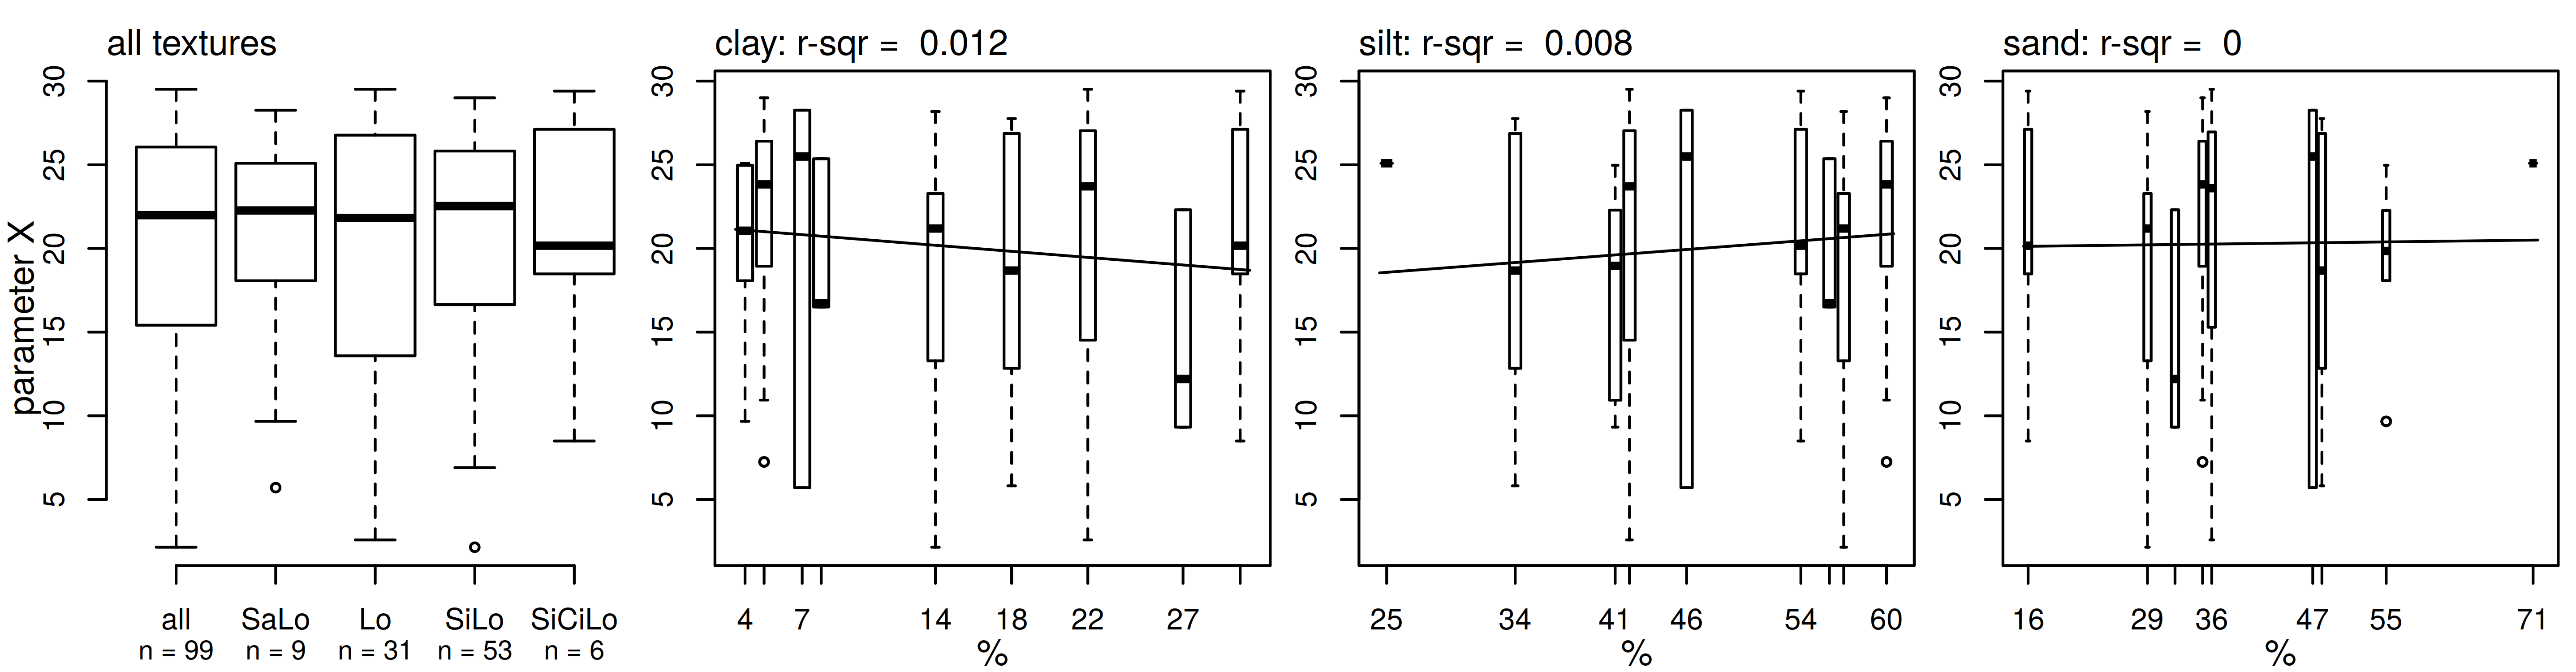
\includegraphics[width = \textwidth]{obr/Xfittex.png}
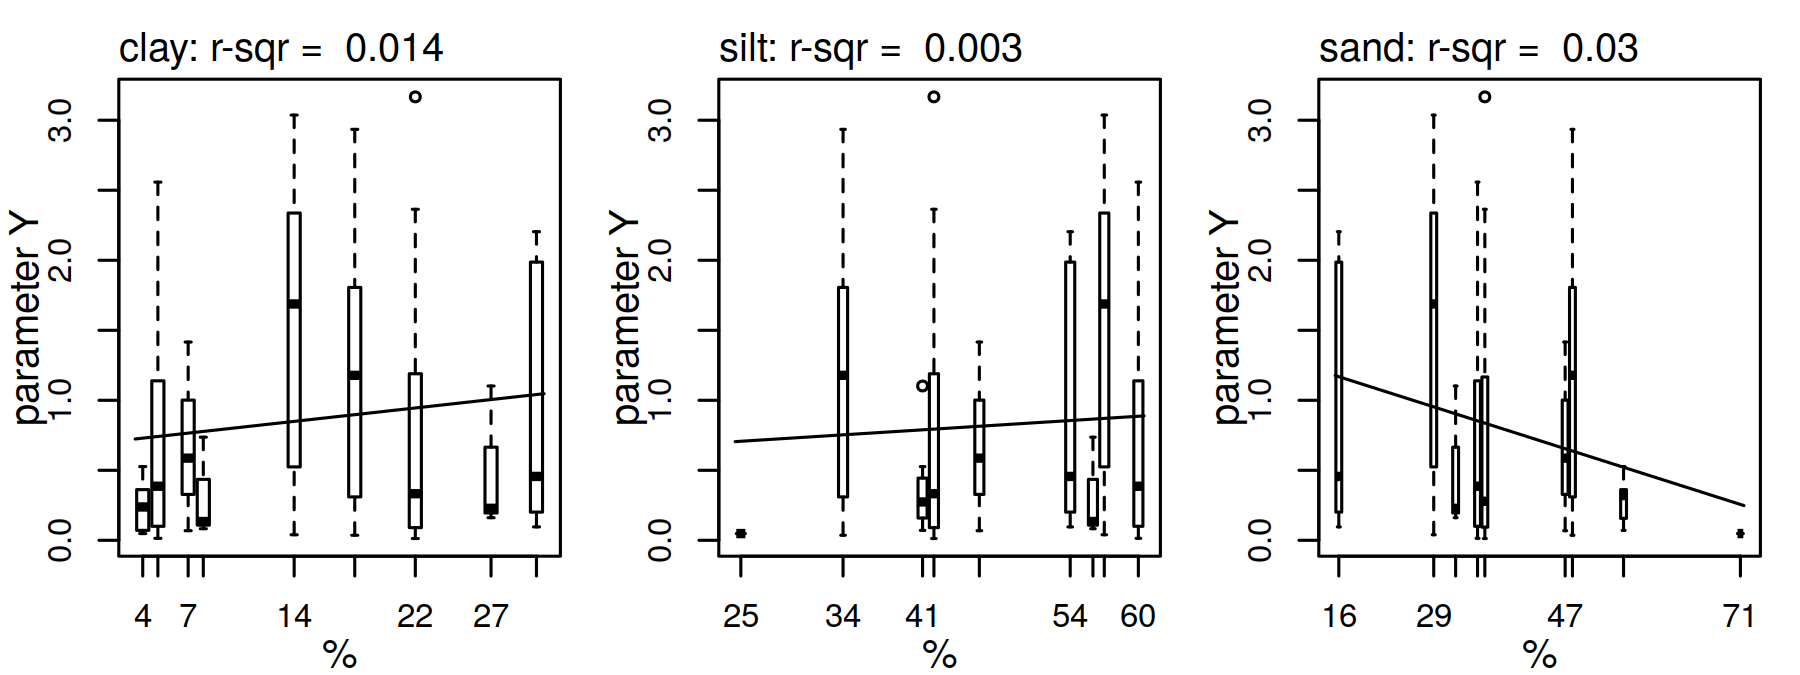
\includegraphics[width = \textwidth]{obr/Yfittex.png}
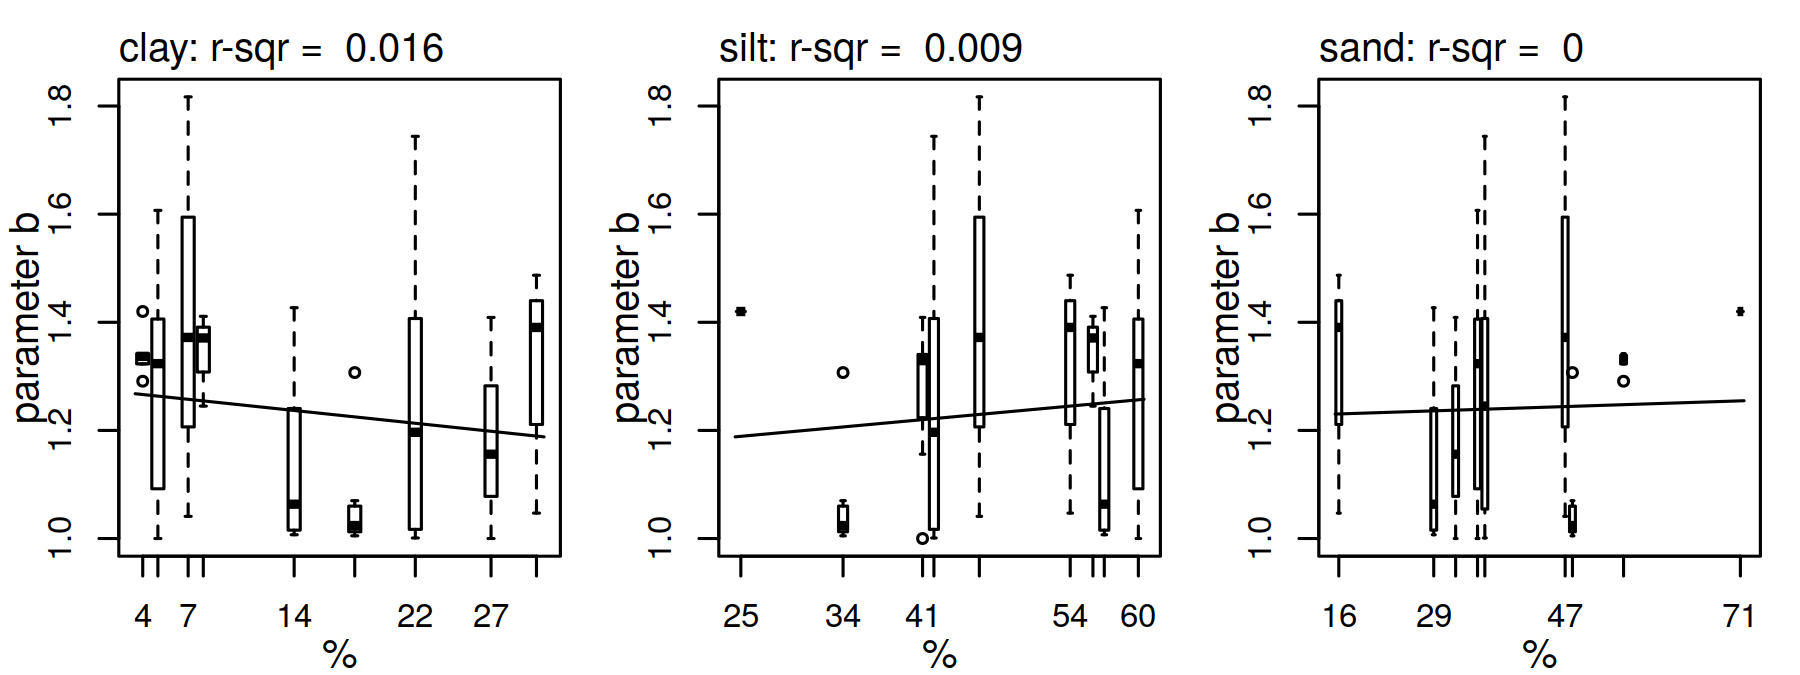
\includegraphics[width = \textwidth]{obr/bfittex.png}
\end{block}



  \end{column}

  \separacnisloupec

  \begin{column}{\threetreti} 
    
\mojesekce{Open source GIS-based implementation}

\justifying
{\rmfamily The SMODERP2D model belongs to a family of so called
GIS-based hydrological models utilizing capabilities of GIS software
for geodata preprocessing. This part is performed by so-called {\em
GIS providers}. Currently there are two GIS providers implemented.

\begin{itemize}
\item originally only proprietary Esri ArcGIS platform (\url{http://desktop.arcgis.com}) supported
\item new generation comes with a provider suited for open source GRASS GIS platform 
\end{itemize}
}

\subsection{GRASS GIS}
\begin{block}{GRASS GIS}
\begin{columns}
    \begin{column}{0.5\textwidth}
    \centering
    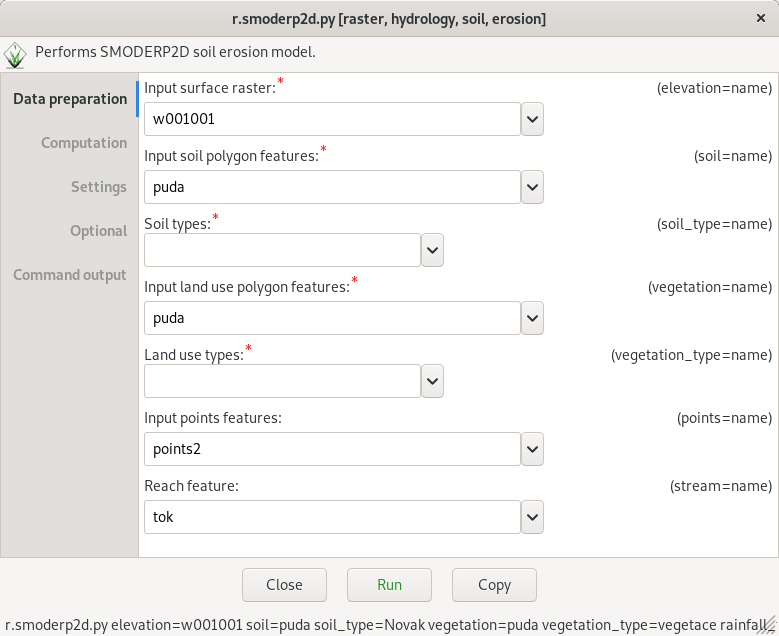
\includegraphics[width = .9\textwidth]{obr/grass.png}
    \end{column}
    \begin{column}{0.5\textwidth}
    
\includegraphics[width = .07\textwidth]{obr/grass-logo.png}
    \justifying
    {\rmfamily {\small
    {\em GRASS} (Geographic Resources Analysis Support System) {\em
    GIS} is a free and open source GIS software suite used for
    geospatial data management and analysis, image processing, spatial
    modeling, and visualization. \newline (\url{http://grass.osgeo.org})}

    \vskip 0.5em

    \begin{itemize}

    \item GRASS-based GIS provider for data preprocessing integrated
    into SMODERP2D codebase
    
    \item {\tt r.smoderp2d} GRASS Addons module for performing
    model computation including data preprocessing

    \end{itemize}
    }
    \end{column}
\end{columns}
\end{block}
\subsection{QGIS}
\begin{block}{QGIS}
\begin{columns}
    \begin{column}{0.5\textwidth}
    
\includegraphics[width = .07\textwidth]{obr/qgis-logo.png}    
    \justifying
    {\rmfamily {\small
    QGIS is a widely known free and open source cross-platform desktop
    geographic information system (GIS) application.}

    \vskip 0.5em

    \begin{itemize}
    
    \item A new QGIS plugin brings the model into QGIS environment
    while data preprocessing part is performed by integrated
    GRASS-based GIS provider
    
    \item QGIS plugin significantly increases accessibility of the
    SMODERP2D model for research purposes and also for engineering
    practice

    \end{itemize}
    
    }

    \end{column}
    \begin{column}{0.5\textwidth}
    \centering
    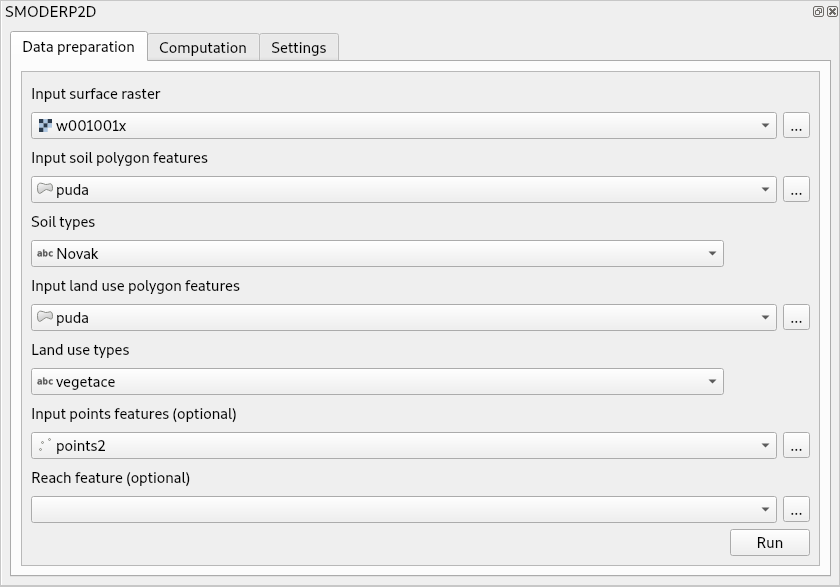
\includegraphics[width = .9\textwidth]{obr/qgis.png}
    \end{column}
\end{columns}
\end{block}

\mojesekce{Conclusions \& Results}
%  \begin{wrapfigure}[8]{r}{0.55\textwidth}
\begin{columns}
    \begin{column}{0.5\textwidth}
        \justifying
        {\rmfamily
        \begin{itemize}
            \item Model is not sensitive to parameter X
            \item Value of newly derived par. b is lower compared with previous inference
            \item Value of parameter Y corresponds to the previous inference
            \item Soil fractions and textural classes explain only a small portion of parameter variation
            \item New generation of SMODERP2D model comes with Esri and GRASS-based GIS providers
        \end{itemize}

        }
    \end{column}
    \begin{column}{0.5\textwidth}
        \justifying
        {\rmfamily
        \begin{itemize}
            \item Accessible via ArcToolbox, GRASS Addons or QGIS plugin
        \end{itemize}
        }
    powered by
    {\tiny
    \begin{lstlisting}
       @ @ @   @       @     @ @     @ @ @     @ @ @ @  @ @ @    @ @ @
      @        @ @   @ @   @     @   @     @   @        @     @  @     @
      @        @   @   @  @       @  @      @  @        @     @  @     @
        @ @    @       @  @       @  @      @  @ @ @    @ @ @    @ @ @
            @  @       @  @       @  @      @  @        @   @    @
            @  @       @   @     @   @     @   @        @    @   @
       @ @ @   @       @     @ @     @ @ @     @ @ @ @  @     @  @

      \  \  /   / /    \   \  /   \  /    /     /        @ @ @   @ @ @
       \ _\/   /_/      \   \/     \/    /_____/        @     @  @     @
           \__/          \  /      _\___/                     @  @      @
               \____      \/      /                          @   @      @
                    \_____/______/                         @     @      @
                                 \                       @       @     @
                                  \____________________ @ @ @ @  @ @ @
    \end{lstlisting}
    }

    \end{column}
\end{columns}


\mojesekce{References}
\justifying
% \small{
{\rmfamily
% \small{
\bibliography{lit}\vspace{0.4cm}
SMODERP2D source code is licensed under GNU
GPL (\url{https://github.com/storm-fsv-cvut/smoderp2d})
% }
}

\mojesekce{Acknowledgment}
\begin{columns}
    \begin{column}{0.4\textwidth}
        \justifying
        {\rmfamily
        The research has been supported by the research grants
        TJ01000270,
        QK1910029,
        and internal CTU grant SGS17/173/OHK1.
        }
    \end{column}
    \begin{column}{0.6\textwidth}
        \centering
        
\includegraphics[height = 5cm]{obr/logo_TACR_dopln_AJ.png}
        
\includegraphics[height = 5cm]{obr/LogoMZeAJ.jpg}
    \end{column}
\end{columns}




% %     \begin{column}{0.4\textwidth}
%     powered by
%     {\tiny
%     \begin{lstlisting}
%        @ @ @   @       @     @ @     @ @ @     @ @ @ @  @ @ @    @ @ @
%       @        @ @   @ @   @     @   @     @   @        @     @  @     @
%       @        @   @   @  @       @  @      @  @        @     @  @     @
%         @ @    @       @  @       @  @      @  @ @ @    @ @ @    @ @ @
%             @  @       @  @       @  @      @  @        @   @    @
%             @  @       @   @     @   @     @   @        @    @   @
%        @ @ @   @       @     @ @     @ @ @     @ @ @ @  @     @  @
% 
%       \  \  /   / /    \   \  /   \  /    /     /        @ @ @   @ @ @
%        \ _\/   /_/      \   \/     \/    /_____/        @     @  @     @
%            \__/          \  /      _\___/                     @  @      @
%                \____      \/      /                          @   @      @
%                     \_____/______/                         @     @      @
%                                  \                       @       @     @
%                                   \____________________ @ @ @ @  @ @ @
%     \end{lstlisting}
%     }
%     \end{column}
% \end{columns}




  \end{column}
  
  \begin{column}{\sepwid}\end{column}
  
  \end{columns}
  \hfill {\tiny The latex template used to create this poster was made by Computational Physics and Biophysics Group, Jacobs University\\[-18pt] \hfill under the licence: CC BY-NC-SA 3.0 (http://creativecommons.org/licenses/by-nc-sa/3.0/)}
  \end{frame} % End of the enclosing frame


\end{document}
